\documentclass[a4paper]{article}
\usepackage{amsfonts}
\usepackage{amsmath}
\usepackage{amssymb}
\usepackage{graphicx}     

\begin{document}
  
\noindent \large Auteur: Shahin Jamal \\
\noindent \large Studierichting: Informatica\\
\noindent \large Oefeningenreeks 5G nr. 6.3\\

\medskip

\normalsize


Bereken het volume $V$ dat men bekomt door het gebied tussen de volgende functies tussen hun snijpunten om
de $X$-as te wentelen.\\

$f(x) = 5x$ en $g(x) = x^2+2x+2$\\

Snijpunten: $5x = x^2+2x+2 \Rightarrow x \in \left\{\dfrac{1}{2}, 2\right\}$\\

$V = \pi  \displaystyle\int\limits_1^2 \left(25x^2 - \left(x^2+2x+2\right)^2\right)dx =  \pi\displaystyle\int\limits_1^2 \left(25x^2 - x^4 - 4x^3 - 8x^2 - 8x - 4\right)dx$\\

$= \pi  \displaystyle\int\limits_1^2 \left(-x^4 - 4x^3 + 17x^2 - 8x - 4\right)dx$\\

$= \pi \left[-\dfrac{x^5}{5}-x^4+\dfrac{17x^3}{3}-4x^2-4x\right]_1^2 = \dfrac{37\pi}{15}$\\

\begin{figure}[h]
\centering
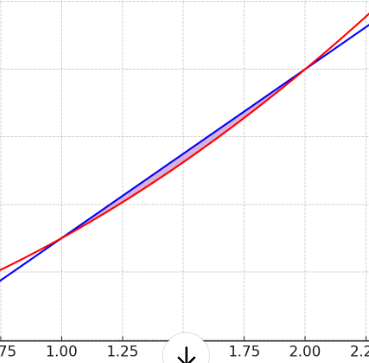
\includegraphics[width=7cm]{5G-6_3_shahin_jamal_INF.png}
\end{figure}

\begin{thebibliography}{999}
%\bibitem{a} Referentie
\end{thebibliography}
\end{document} 
